\documentclass{tikzposter}
\geometry{paperwidth=24in, paperheight=36in}

% 2 feet wide by 3 feet tall
% 24in=2ft, 36in=3ft

% 3 feet wide by 4 feet tall
% 36in=3ft, 48in=4ft

\makeatletter
\setlength{\TP@visibletextwidth}{22in}
\setlength{\TP@visibletextheight}{34in}
\makeatother

\usepackage[utf8]{inputenc}
\usepackage{tikz}
\usepackage{xcolor}

\usepackage{setspace}
\onehalfspacing

\usepackage[pangram]{blindtext}
\usepackage{comment}
\usetikzlibrary{arrows.meta}
\usepackage{minted}

\newcommand{\largearrow}{-{Latex[length=3mm,width=5mm]}}

% Colors sourced from https://www.redcross.org/content/dam/redcross/atg/PDFs/BrandPoster.pdf
\definecolor{coolgray}{HTML}{6D6E70}
\definecolor{redcrossred}{HTML}{ED1B2E}

\tikzset{%
  >={Latex[width=2mm,length=2mm]},
  % Specifications for style of nodes:
            base/.style = {rectangle, rounded corners, draw=black,
                           minimum width=8cm, minimum height=1cm,
                           text centered, font=\sffamily},
		startstyle/.style = {base, fill=blue!30},
		astyle/.style = {base, fill=red!30},
		bstyle/.style = {base, fill=green!30},
		cstyle/.style = {base, minimum width=2.5cm, fill=orange!15,
                           font=\ttfamily},
}

\usecolorstyle[colorOne=coolgray,colorTwo=white,colorThree=redcrossred]{Germany}
\tikzposterlatexaffectionproofoff

\title{Twitter Fire Scraper}
\author{Coding Team}
\date{\today}
\institute{Illinois Institute of Technology}

\begin{document}

\maketitle

\begin{columns}

\column{1}
\block{Overview}
{
    {
    \fontsize{36pt}{14pt}\selectfont
    Twitter has become one of the most influential forms of social media in the last decade. Its users include some of the highest profiled politicians, businessmen, artists, and celebrities. Twitter is also a reliable source of first-hand information. Our team presents the Twitter Fire Scraper, a tool that can scrape through a large amount of tweets in a matter of seconds, specified by either keywords or usernames. In our project, we use the scraper to identify fire incidents, allowing us to quickly and efficiently provide vital information to the American Red Cross.     
    }
}


\end{columns}


\begin{columns}

    \column{0.5}
    \block{Screenshots}
    {
        \begin{tikzfigure}
            [
                Twitter Fire Scraper Web API Console
            ]
            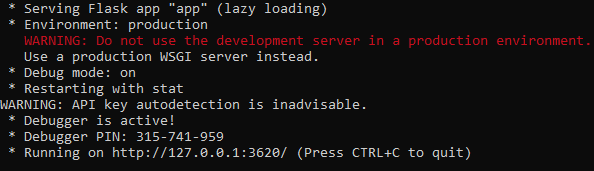
\includegraphics[width=0.3\textwidth]{webapi_console.PNG}
            
        \end{tikzfigure}

        \begin{tikzfigure}
            [
                Twitter Fire Scraper Dashboard Console
            ]
            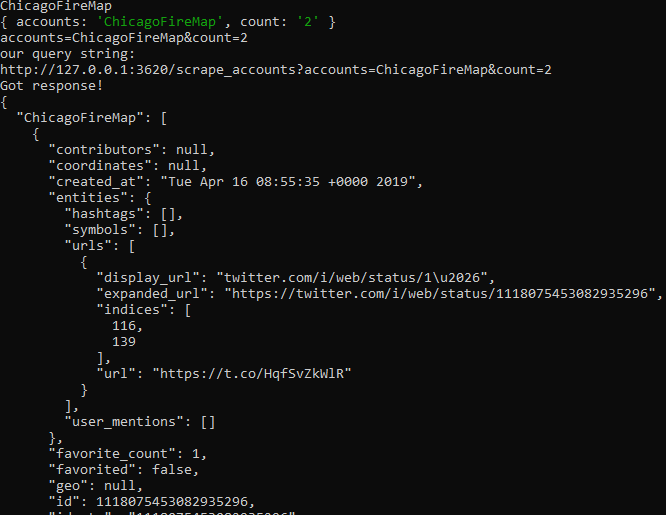
\includegraphics[width=0.3\textwidth]{chicagofire_console.png}

        \end{tikzfigure}

        \begin{tikzfigure}
            [
                Twitter Fire Scraper Dashboard Web Interface
            ]
            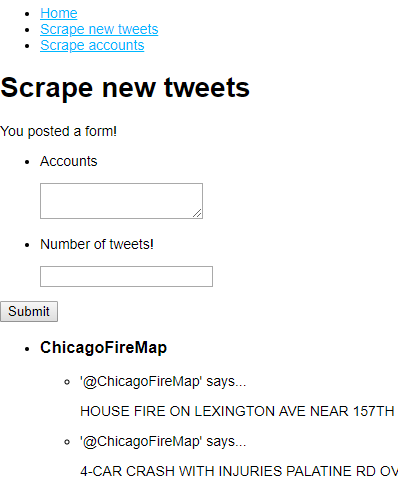
\includegraphics[width=0.3\textwidth]{chicagofire.png}
            
        \end{tikzfigure}
    }

    \column{0.5}
    \block{Application Diagram}
    {
        \begin{tikzfigure}%[Caption]
            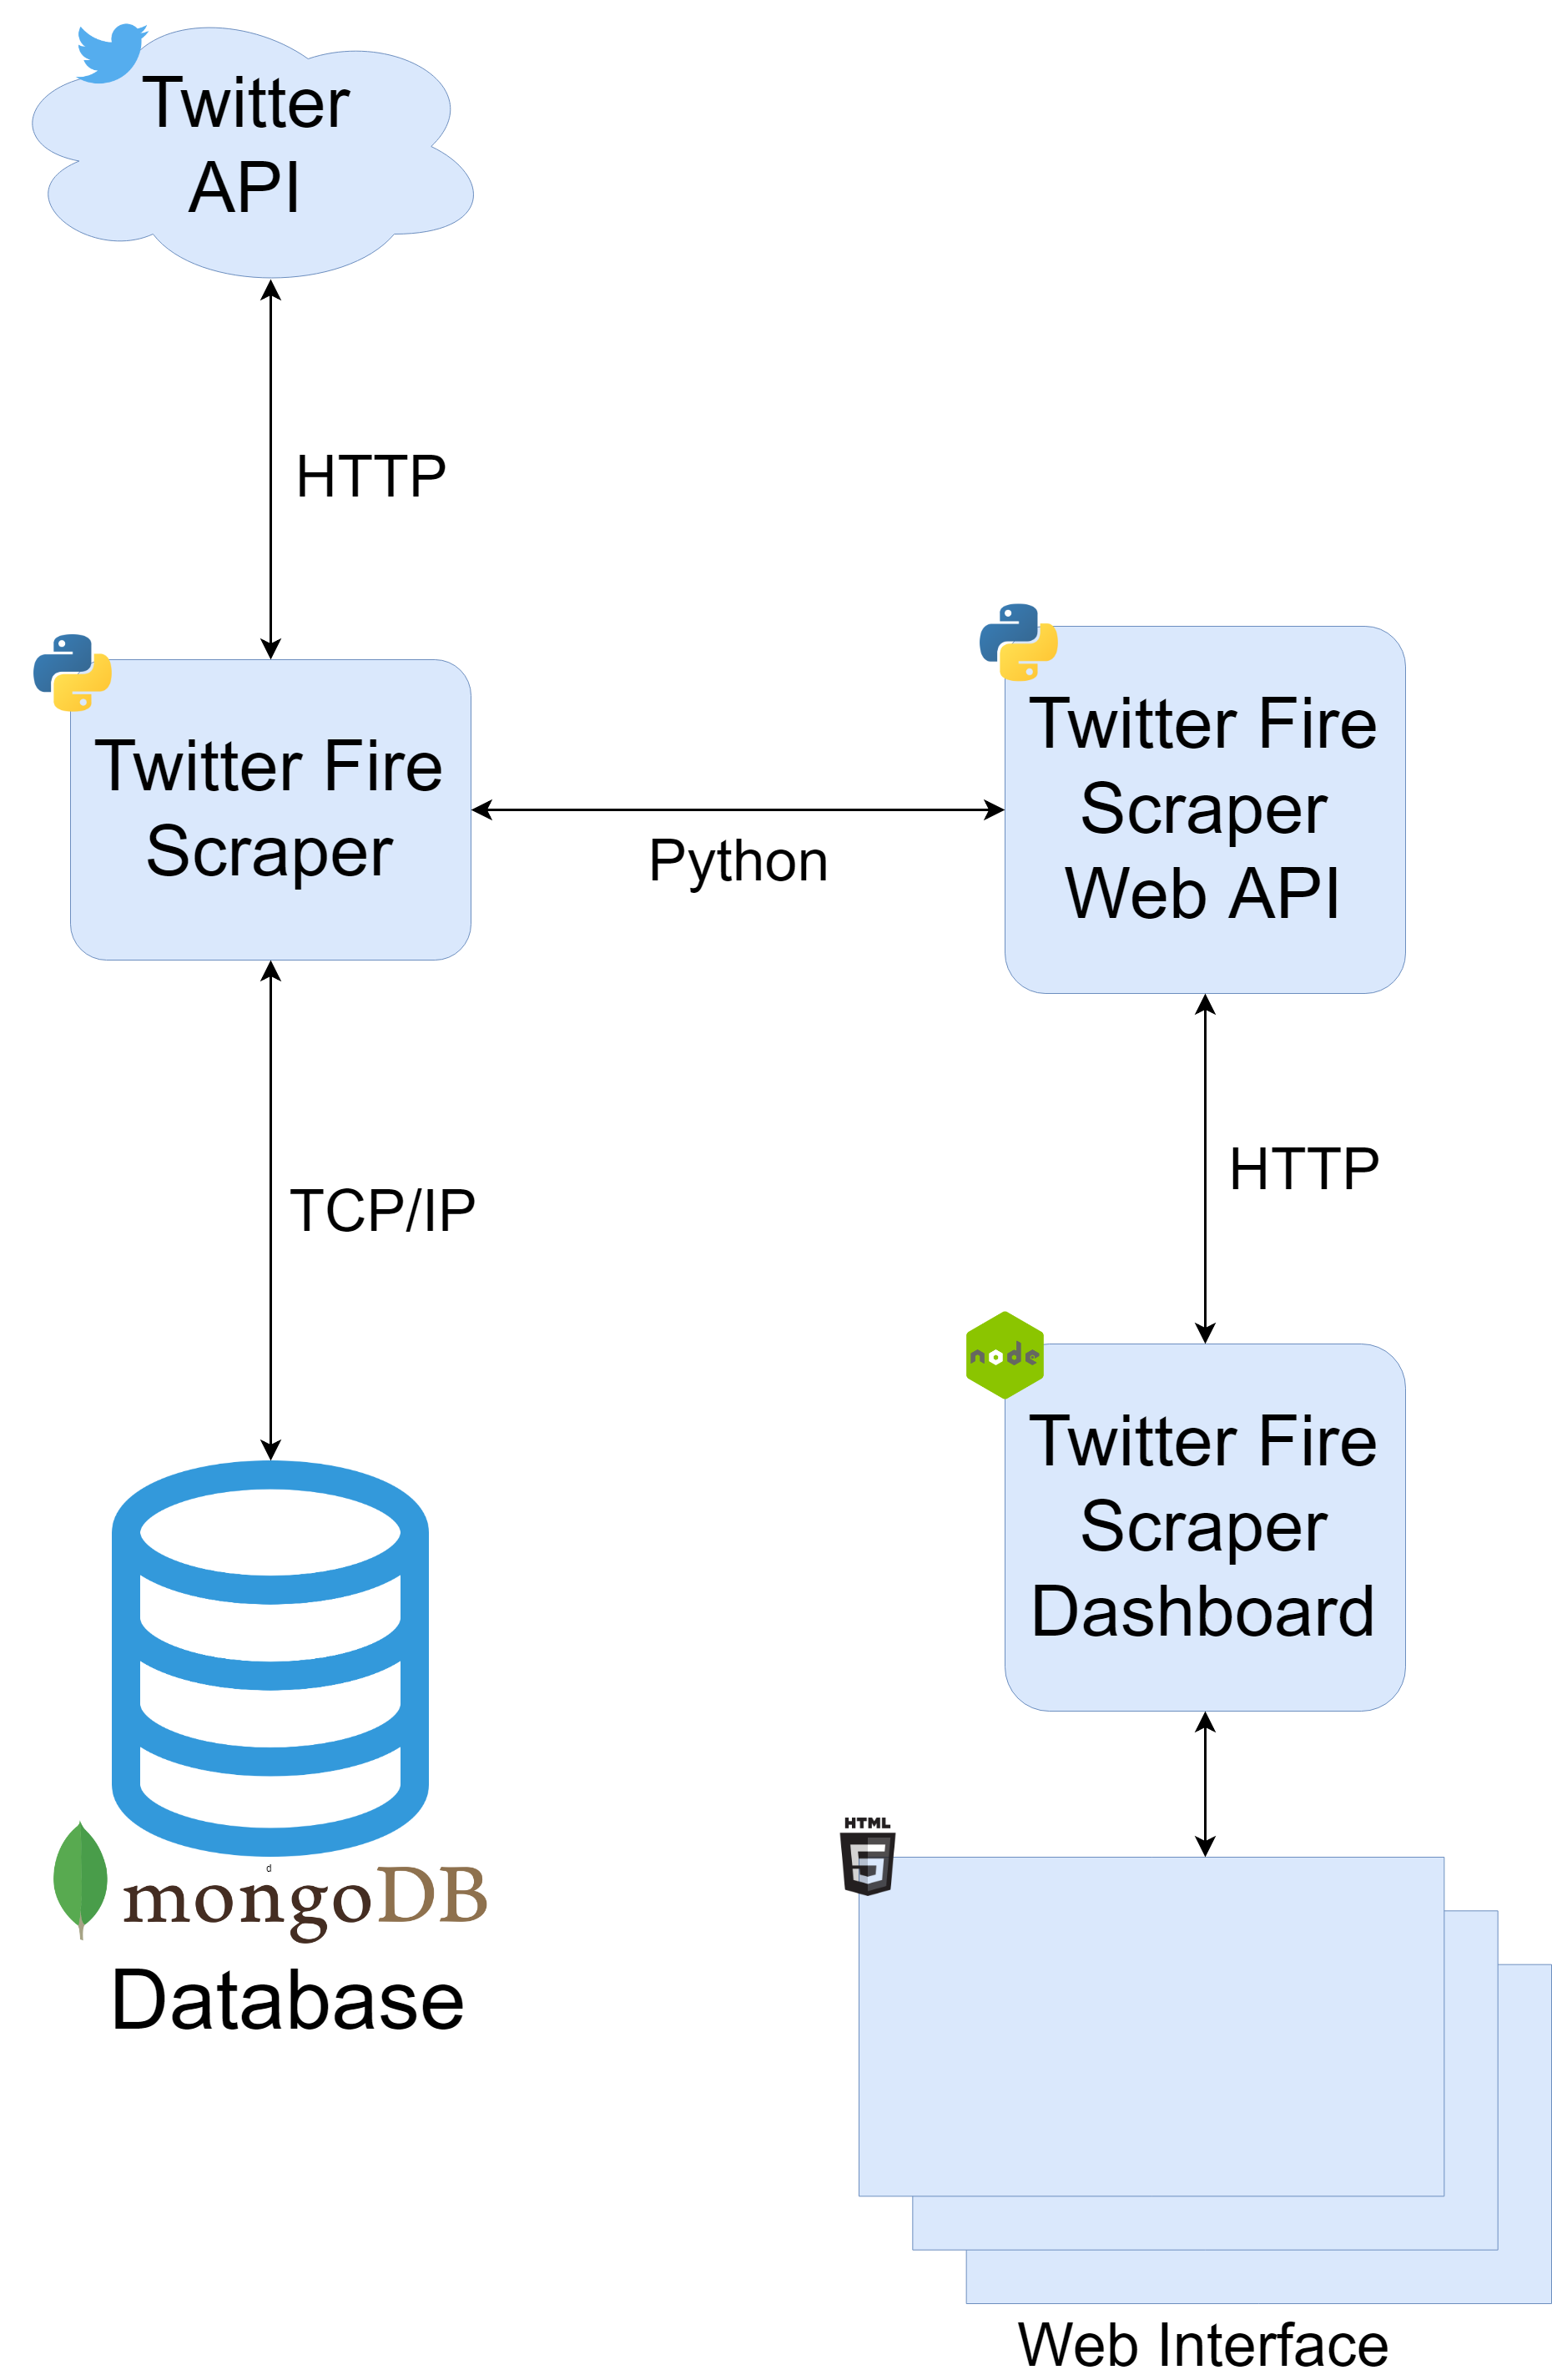
\includegraphics[width=0.3\textwidth]{application-diagram.png}
        \end{tikzfigure}
        {
        \fontsize{36pt}{14pt}\selectfont
        The Twitter Fire Scraper utilizes Twitter's API to collect an account's tweets, or to search Twitter for key terms. The scraper can then save those tweets to a mongoDB database or to an Excel file, which can be easily accessed. In order to make the scraper accessible through a web interface, a Web API for the Twitter Fire Scraper accepts terms and amount of tweets to search for. The Dashboard connects to the Web API via Node.js, and then brings the data from the scraper to the Web Interface.
        }
    }
    
    \block{}% Logos
    {
        \vspace{-2.5cm}
        \begin{tikzfigure}[]
        
\includegraphics[scale=0.4]{Logos.png}
        \end{tikzfigure} 
    }

    
\end{columns}

\end{document}
